\chapter{\ifproject%
    \ifenglish Project Structure and Methodology\else โครงสร้างและขั้นตอนการทำงาน\fi
  \else%
    \ifenglish Project Structure\else โครงสร้างของโครงงาน\fi
  \fi
 }

ในบทนี้จะกล่าวถึงหลักการ และการออกแบบระบบ

\makeatletter

% \renewcommand\section{\@startsection {section}{1}{\z@}%
%                                    {13.5ex \@plus -1ex \@minus -.2ex}%
%                                    {2.3ex \@plus.2ex}%
%                                    {\normalfont\large\bfseries}}

\makeatother
%\vspace{2ex}
% \titleformat{\section}{\normalfont\bfseries}{\thesection}{1em}{}
% \titlespacing*{\section}{0pt}{10ex}{0pt}
% \begin{figure}
% \begin{center}
% 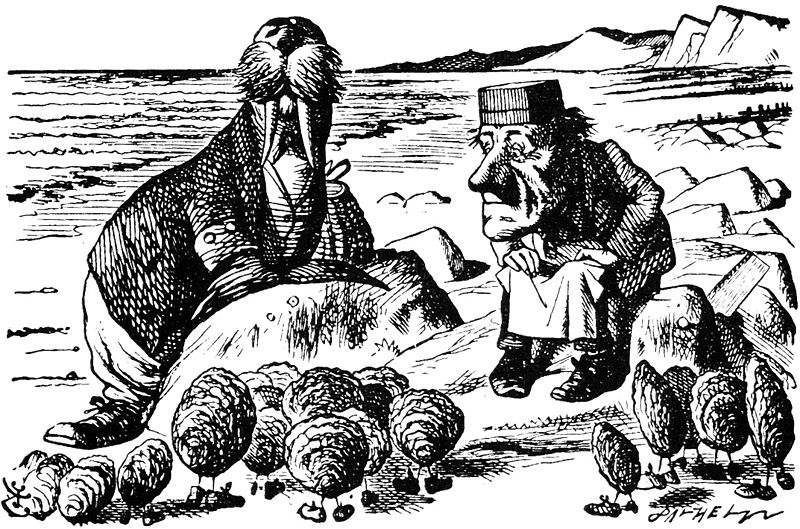
\includegraphics{photo.old/800px-Briny_Beach.jpg}
% \end{center}
% \caption[Poem]{The Walrus and the Carpenter}
% \label{fig:walrus}
% \end{figure}

\section{ภาพรวมของแอพพลิเคชัน}

% เว็บแอพพลิเคชันจะเป็นแบบ three-tier architecture แต่ว่าจะทำการออกแบบ และพัฒนาให้สามารถรองรับการเปลี่ยนแปลงเป็น 
% microservice ได้ โดย Front-end และ Back-end ส่วนมากจะพัฒนาด้วย Next.js และ tRPC เพื่อความสะดวกสบายในการเรียกใช้งาน API
% และใช้ typescript ให้มีประสิทธิภาพ แต่ Back-end ในส่วนของระบบจับคู่นั้นจะพัฒนาด้วย Go เพราะสามารถเขียน concurrency ได้ง่ายแต่ยังคงไว้ซึ่งประสิทธิภาพ
% ส่วนสุดท้ายคือฐานข้อมูลจะใช้ postgresql ในการจัดเก็บและติดต่อกับ Back-end ทั้ง Next.js และ Go

เว็บแอพพลิเคชันจะเป็นแบบ three-tier architecture แต่จะทำการออกแบบ และพัฒนาให้สามารถรองรับการเปลี่ยนแปลงเป็น microservice ได้ โดย frontend 
และ backend จะพัฒนาด้วย Next.js ,TypeScript และ tRPC ซึ่งมีส่วนช่วยให้การพัฒนามีความถูกต้องจากตัวแปรของทั้ง backend และ frontend เพราะอัลกอริทึมมีอินพุตที่ต้องการเป็นจำนวนมาก
และมีหลายส่วนย่อยเมื่อมีการเรียกใช้งานข้ามไปมา ถ้าไม่มีการจำกัดประเภทตัวแปรที่ต้องส่งจะทำให้เกิดข้อผิดพลาดเป็นจำนวนมาก
ส่วนสุดท้ายคือฐานข้อมูลจะใช้ PostgreSQL ในการจัดเก็บและติดต่อกับ backend

% เว็บแอพพลิเคชันใช้ three-tier architecture~\cite{ttarch} ในการออกแบบระบบ โดย front-end ใช้ Next.js\cite{nextjs} 
% ที่เป็น React~\cite{react} framework ส่วน back-end ใช้ Gin Gonic~\cite{gingonic} ซึ่งเป็น Go~\cite{golang} framework ติดต่อกับ Front-end 
% ด้วย GraphQL~\cite{graphql} API และฐานข้อมูลใช้ MySQL~\cite{mysql} เป็น relational database management system (RDBMS)

\begin{figure}[h]
  \begin{center}
    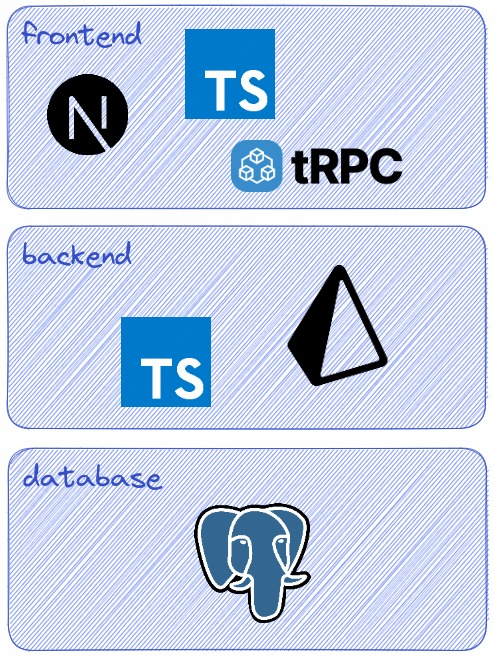
\includegraphics[width=2.5in]{photo/diagram/app-arch.jpeg}
  \end{center}
  \caption{three-tier architecture}
  \label{fig:three-tier}
\end{figure}

\section{ขั้นตอนการจับคู่}
% ในส่วนของกระบวนการจับคู่นั้น จะแบ่งออกเป็น 3 ขั้นตอนนั่นคือ การระบุความต้องการของผู้ร่วมอาศัย การให้นิยามความคล้ายคลึงกันของรายการความต้องการ
% และการจับคู่ผู้ร่วมอาศัยตามความต้องการ
การจับคู่หารูมเมทที่คู่ควรนั้น โครงการนี้ได้แบ่งขั้นตอนไว้ ด้วยกันทั้งสิ้น 3 ส่วนด้วยกัน นั่นคือ
\begin{enumerate}
  \item preference declaration: การระบุ preference ของรูมเมทหรือห้องที่ต้องการ และ profile ของเจ้าของ preference นั้น 
  \item finetuning: การหาขอบเขตลักษณะของรูมเมทที่พอรับได้ และน้ำหนักความสนใจของแต่ละคุณลักษณะของรูมเมท
  \item matching: การจับคู่จะพิจารณาจากข้อมูลที่ได้ในขั้นตอนที่ $1$ และ $2$
\end{enumerate}

\begin{figure}[h]
  \begin{center}
    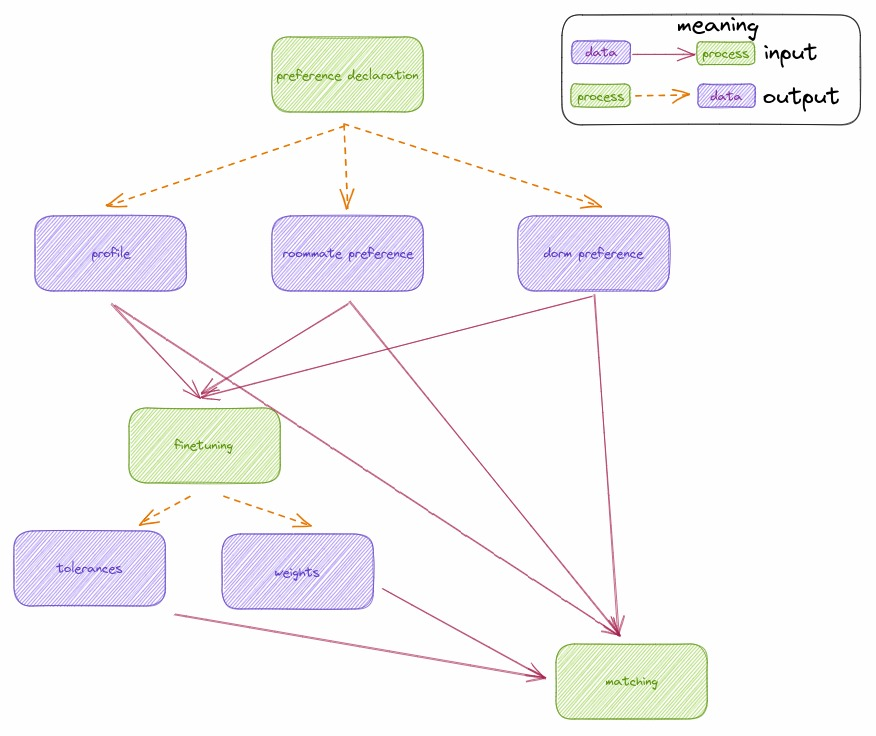
\includegraphics[width=2.5in]{photo/diagram/matching-flow.jpeg}
  \end{center}
  \caption{ภาพรวมของอัลกอริทึม}
  \label{fig:match-overall}
\end{figure}

\subsection{ระบุรายการความต้องการ}
ในขั้นแรกของอัลกอริทึมจะทำการรวบรวมข้อมูลต่างๆ ของผู้ใช้ได้แก่ 
คุณลักษณะของผู้ใช้ คุณลักษณะของผู้ร่วมอาศัยที่ต้องการ ห้องพักที่ต้องการ หอพักที่ต้องการ เรียกว่า $profile$ $matePref$ $roomPref$
และ $dormPref$ ตามลำดับ

\subsection{คำนวณขอบเขตลักษณะของรูมเมทที่พอรับได้}
หลังจากที่ได้ preference ต่างๆครบถ้วนแล้วจะทำการค้นหาขอบเขตลักษณะของรูมเมทที่เจ้าของระบุมา
เนื่องจากอัลกอริทึมนี้ตั้งสมมุติฐานไว้ว่าผู้ใช้นั้นไม่ได้รู้ถึงความต้องการที่แน่ชัดของตนเอง เช่น 
นาย ก บอกว่าอยากได้รูมเมทที่มีการรักษาความสะอาดระดับ 4 ซึ่งจริงๆแล้ว อาจจะยอมรับระดับ 5 ได้ หรืออาจจะไม่ยอมรับรูมเมทที่รักษาความสะอาดมากกว่าตัวเองเช่นระดับ 1
ซึ่งจะหาโดยการให้ผู้ใช้เลือกโปรไฟล์ที่มีการปรับค่า \MEreply{not finished yet}

\subsection{คำนวณน้ำหนักความสนใจของแต่ละคุณลักษณะของรูมเมท}
เพราะผู้ใช้แต่ละคนนั้นมีความสนใจที่แตกต่างกัน บางคนอาจจะสนใจระดับเสียงที่ใช้ในห้องพักมากที่สุด บางคนอาจจะสนใจระดับความสะอาดของรูมเมทมากที่สุด 
จึงต้องทำการค้นหาค่าน้ำหนักที่จะระบุความสำคัญของแต่ละคุณลักษณะของ preference ที่ผู้ใช้ระบุ ว่าผู้ใช้แต่ละคนมีความสนใจคุณลักษณะไหนอย่างไรบ้าง  
ซึ่งอัลกอริทึมการจับคู่จะนำข้อมูลน้ำหนักเหล่านี้ไปใช้ประกอบการจับคู่รูมเมทในขั้นถัดไป โดยวิธีการหาค่าน้ำหนักมีดังนี้


% \subsection{วิธีตัดสินในการจับคู่ตามความต้องการ}
% ระบบจะทำการคำนวณค่าบทลงโทษ(penalty) ตามคุณลักษณะที่ไม่ตรงตามความต้องการ ทำให้ผู้ใช้ที่มีคุณลักษณะไม่ตรงตามความต้องการมีค่า penalty ต่อกันสูง
% โดยค่าคุณลักษณะที่จะใช้พิจารณานั้นปัจจุบันมีอยู่ทั้งสิ้น 2 แบบคือ
% \begin{enumerate}
%   \item แบบค่าสูงสุด คือหากคุณลักษณะมีค่าไม่เกินค่าสูงสุดค่าจะไม่มี penalty ไม่อย่างนั้นค่า penalty จะสูงขึ้นตามส่วนต่างที่เกินมาจากค่าสูงสุด
%   \item แบบช่วง คือหากคุณลักษณะมีช่วงที่ซ้อนทับกับช่วงที่ต้องการพอดีจะไม่มี penalty ไม่อย่างนั้นจำนวนที่ไม่ซ้อนทับกันจะยิ่งเพิ่มค่า penalty
% \end{enumerate}

\subsection{วิธีการคำนวณ penalty}
ในการคำนวณค่า penalty นั้นจำเป็นต้องใช้ข้อมูล 2 ส่วนนั่นคือค่า $w_{attr}$ และ $\Delta attr$ โดย
\begin{enumerate}
  \item $w_{attr}$ คือ weight ของคุณลักษณะที่สนใจ $attr$
  \item $\Delta attr$ คือส่วนต่างระหว่างค่าคุณลักษณะของโปรไฟล์รูมเมท $attr_{profile}$ 
        กับค่าคุณลักษณะของรูมเมทที่เราสนใจ $attr_{roomPref}$ 
\end{enumerate}
ซึ่งค่า weight จะเป็นค่าที่บ่งบอกระดับความสำคัญของคุณลักษณะนั้นๆ ว่าสำคัญมากน้อยเพียงใด ซึ่งค่านี้จะต่างออกไปตามแต่ละบุคคล

\subsection{การหาค่า weight} 
โดยค่า weight นั้นจะได้จากการ

\subsection{เลือกหอให้ผู้ใช้ตามความต้องการ}
ลำดับต่อไปจะเป็นการเลือกหอพักให้กับผู้ใช้ตามความต้องการ เนื่องจากหอพักนักศึกษาของมหาวิทยาลัยเชียงใหม่นั้นมีค่าใช้จ่ายที่ไม่เท่ากัน
และนักศึกษาแต่ละคนมีกำลังในการจ่ายค่าหอพักที่ไม่เท่ากัน จึงจำเป็นที่จะต้องเลือกก่อนการเลือกผู้ร่วมอาศัย 

\subsection{ตัวเลือกต่างๆ ในขั้นตอนเลือกห้องพัก และผู้ร่วมอาศัย}
เนื่องจากในส่วนก่อนหน้าที่ระบุไว้ว่าปัญหาการจับคู่นี้เป็น NP-complete จึงจำเป็นที่จะต้องหาทางเลือกอื่นในการพัฒนา 
ซึ่งในปัจจุบันสามารถแบ่งออกได้เป็น 3 แบบนั่นคือ
\begin{enumerate}
  \item เลือกผู้พักอาศัยก่อนเลือกห้องพัก
        วิธินี้จะเลือกและจัดกลุ่มของผู้พักอาศัยตามจำนวนผู้พักอาศัยใน 1 ห้องของหอพัก โดยวิธีการเลือกนั้นจะเลือกจากผู้ใช้ที่มีค่า penalty ต่อกันน้อยที่สุด
        แล้วจากนั้นแต่ละกลุ่มจะทำการเลือกห้องพักโดย penalty คิดจากผลรวมของ penalty ที่ได้จาก $roomPref$ ของสมาชิกในกลุ่ม
        ซึ่งวิธินี้จะทำให้นักศึกษาได้เพื่อนร่วมห้องที่ต้องการ แต่อาจจะทำให้นักศึกษาบางคนในกลุ่มไม่ได้ห้องพักตามที่ต้องการ
  \item เลือกกลุ่มของห้องพักก่อนเลือกผู้พักอาศัย
        วิธีนี้จะเลือกและจัดกลุ่มของนักศึกษาเข้าไปในกลุ่มของห้องพักก่อน โดยในแต่ละกลุ่มของห้องจะเป็นห้องที่มีลักษณะเหมือนๆกัน
        หลังจากนั้นจะทำการจับกลุ่มของนักศึกษาให้เข้ากับแต่ละห้องในกลุ่ม ซึ่งวิธีนี้จะทำให้นักศึกษาได้ห้องที่ใกล้เคียงความต้องการมากที่สุด 
        แต่จะทำให้ห้องบางห้องมีนักศึกษาที่ไม่เหมาะสมที่จะจับคู่กันเกิดขึ้น
  \item พิจารณาเลือกทั้งห้องพักและผู้พักอาศัยพร้อมๆ กัน
        วิธีนี้จะทำการคิด penalty ของทั้ง $roomPref$ และ $matePref$ พร้อมๆ กันโดยเอาค่า $roomPref + matePref$ เป็น penalty
        แต่ผู้พัฒนายังไม่สามารถหาวิธีที่จะทำการเลือกลำดับนักศึกษาที่แน่นอน ในการจับคู่ผู้ร่วมอาศัยและห้องพักพร้อมๆ กัน
\end{enumerate}

ซึ่งวิธีทั้ง 3 นั้นยังไม่สามารถยืนยันได้ว่าจะใช้แบบใด เพราะปัจจุบันยังอยู่ในขั้นตอนของการศึกษาค้นคว้าเพิ่มเติม
% \subsection{ตัวอย่างการทำงาน}
% \begin{enumerate}
%   \item นำลำดับคุณลักษณะที่ผู้ใช้ $u$ จัดอันดับไปแปลงเป็นตัวเลขเพื่อใช้เป็นตัวคูณในขั้นตอนต่อๆไป โดยเรียกตัวคูณนั้นว่า $\mathit{mult}$
%   \item เก็บรายการคุณลักษณะที่ผู้ใช้พิจารณาเพื่อนร่วมห้องจากการจัดลำดับในขั้นตอนก่อนหน้าแล้วเรียกว่า $\mathit{attr}$
%   \item ปรับปรุง $\mathit{mult}$ เพิ่มเติมในขั้นตอนการปรับจูน หากคุณลักษณะใดที่ผู้ใช้ให้ความสนใจบ่อยๆ จะถูกเพิ่มค่าให้มากขึ้น และคุณลักษณะใดที่ผู้ใช้ไม่ให้ความสนใจก็จะถูกลดค่าให้น้อยลง 
%         เช่น หากมีโปรไฟล์ที่มีคุณลักษณะดังนี้
%         \begin{enumerate}
%           \item เวลานอนช่วง 4 ทุ่ม -- 5 ทุ่ม และ เป็นคนช่างพูด  
%           \item เวลานอนช่วง 4 ทุ่ม -- 5 ทุ่ม และ เป็นคนพูดน้อย  
%         \end{enumerate} 
%         แล้วผู้ใช้เลือกทั้งสองโปรไฟล์นั้น ดังนั้นระบบจะทำการปรับเพิ่มค่าในตัวคูณของคุณลักษณะเวลานอนใน $\mathit{mult}$
%   \item นำ $\mathit{mult}$ ไปคูณกับค่าของคุณลักษณะของผู้ใช้ $v$ คนอื่นๆที่ไม่ใช่ $u$ แล้วบวกผลคูณทั้งหมดเข้าด้วยกัน เรียกว่า $\mathit{RoommatePref}$
%   \item ทำแบบข้อก่อนหน้ากับคุณลักษณะของห้องพักที่ต้องการ และ คุณลักษณะตามโปรไฟล์ของผู้ใช้ $u$ เรียกว่า $\mathit{RoomPref}$ และ $\mathit{PersonalPref}$ ตามลำดับ
%   \item สร้างคู่อันดับ $(\mathit{RoomPref}, \mathit{RoommatePref})$ จากค่าของผู้ใช้ เรียกว่า $(x,y)$ 
%   \item สร้างคู่อันดับ $(\mathit{RoomPref}, \mathit{PersonalPref})$ ของผู้ใช้คนอื่น เรียกว่า $(x',y')$
%   \item หาคู่อันดับ $(x',y')$ ที่มีระยะทางแบบยูคลิด~\cite{euclid-dist} จาก $(x,y)$
%   \[\sqrt{(x-x')^2 + (y-y')^2}\] มีค่าน้อยที่สุด 
%   แล้วให้ $(x',y')$ ของผู้ใช้คนนั้นคู่เป็นเพื่อนร่วมห้อง
% \end{enumerate}

\MEreply{เป็นช่วง8.1 ของ NSC อาจจะทำรูป flow คร่าวๆ}
\section{User story}
ต่อไปจะเป็นการอธิบายการทำงานของระบบในส่วนต่างๆ ทั้งฝั่งผู้ใช้งานทั่วไปและผู้ดูแลระบบ โดยรูปภาพตัวอย่างต่อไปนี้เป็นเพียง wireframes เท่านั้น ไม่ใช่ user interface ของระบบจริง
\subsection{นักศึกษา}
\begin{enumerate}
  \item นักศึกษาเข้าสู่หน้าต้อนรับของแอพพลิเคชัน แต่ยังไม่สามารถทำอะไรได้ ต้องทำการยืนยันตัวตนด้วยการคลิกปุ่ม login หรือ quick start ก่อน
        \begin{figure}[h]
          \begin{center}
            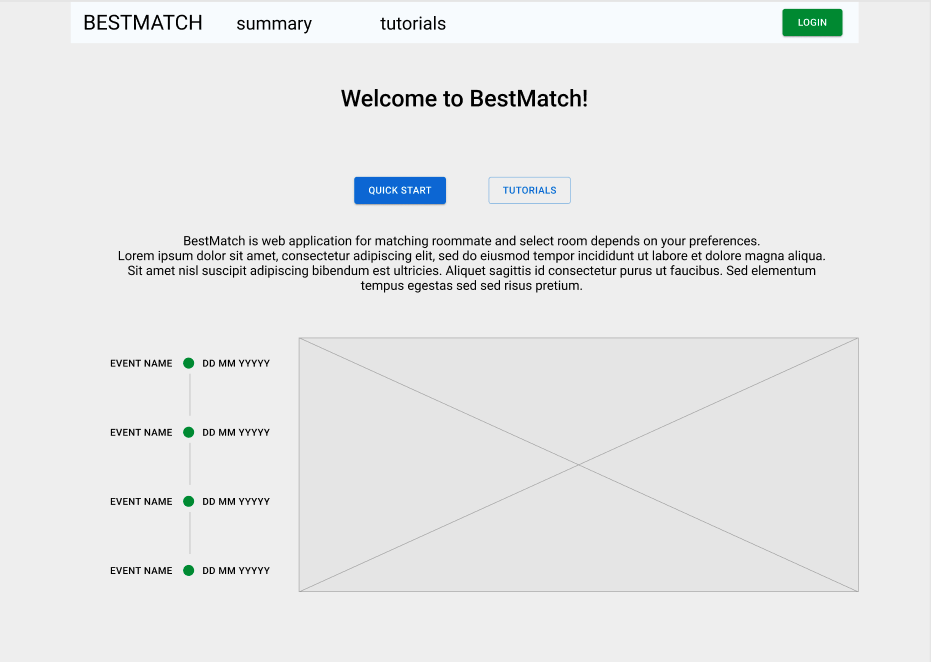
\includegraphics[width=\linewidth]{photo/student/home.png}
          \end{center}
          \caption{หน้าต้อนรับที่ไม่ได้ยืนยันตัวตน}
          \label{fig:homepage}
        \end{figure}
        \clearpage
  \item นักศึกษายืนยันตัวตน โดยหน้าต่างล็อคอิน ซึ่งสามารถสร้างบัญชีใหม่ได้หากยังไม่มีบัญชี ดังรูปตัวอย่าง
        \begin{figure}[h]
          \begin{center}
            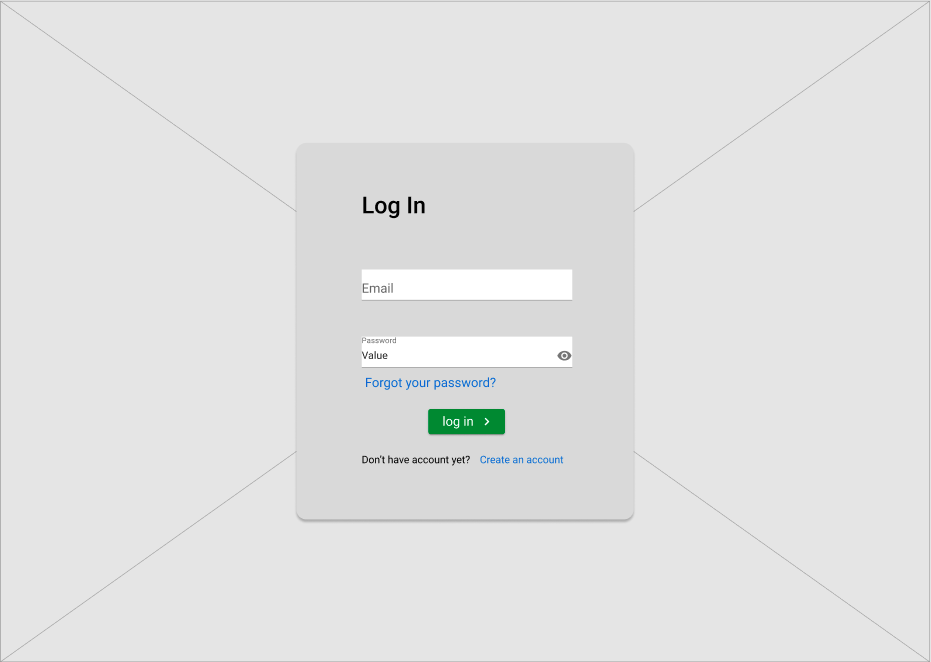
\includegraphics[width=\linewidth]{photo/student/login.png}
          \end{center}
          \caption{หน้าต่างล็อคอิน}
          \label{fig:login}
        \end{figure}
        
        \begin{figure}[h]
          \begin{center}
            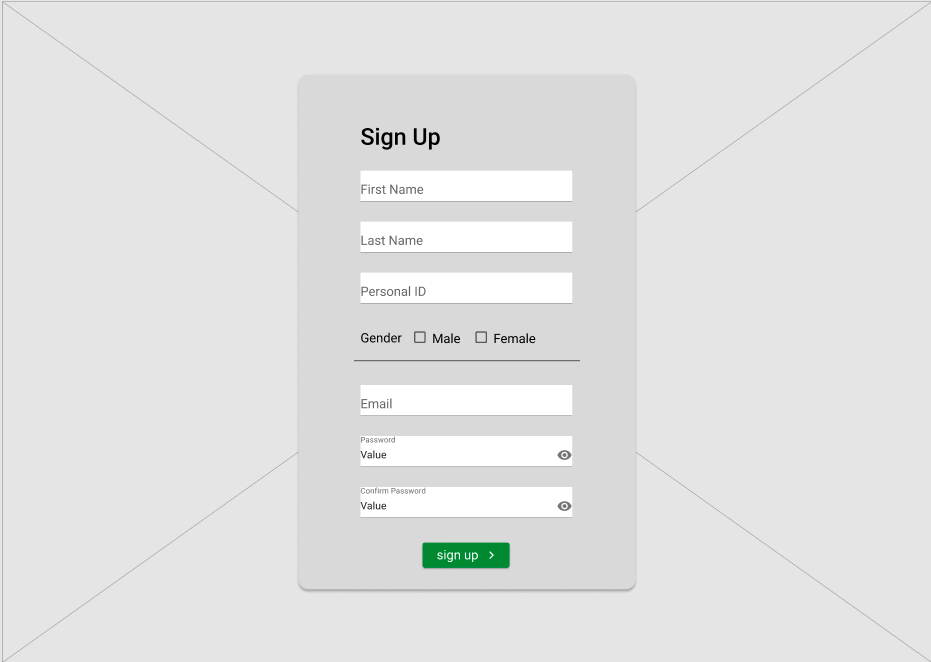
\includegraphics[width=\linewidth]{photo/student/register.png}
          \end{center}
          \caption{หน้าต่างลงทะเบียน}
          \label{fig:register}
        \end{figure}
        
        \begin{figure}[h]
          \begin{center}
            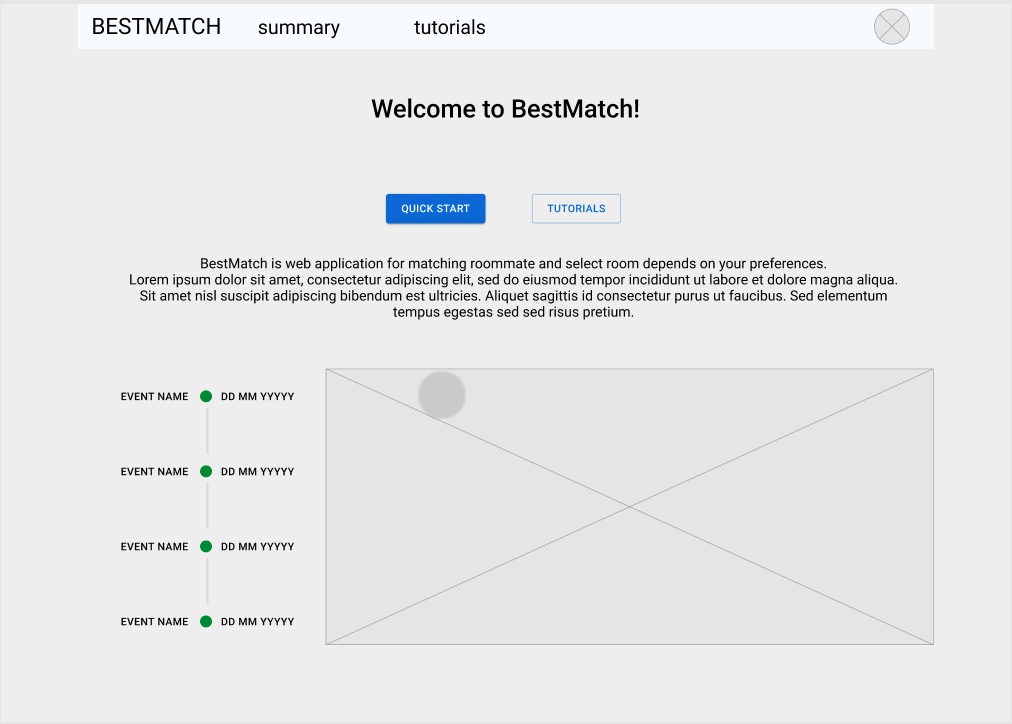
\includegraphics[width=\linewidth]{photo/student/home-auth.png}
          \end{center}
          \caption{หน้าต้อนรับหลังจากการยืนยันตัวตน}
          \label{fig:homepage-auth}
        \end{figure}
        \clearpage
  \item นักศึกษาเรียนรู้การทำงานด้วยหน้าต่างคู่มือการใช้งาน ซึ่งจะมีแผนผังที่สามารถมีปฏิสัมพันธ์ในการช่วยแนะนำแอพพลิเคชัน
        \begin{figure}[h]
          \begin{center}
            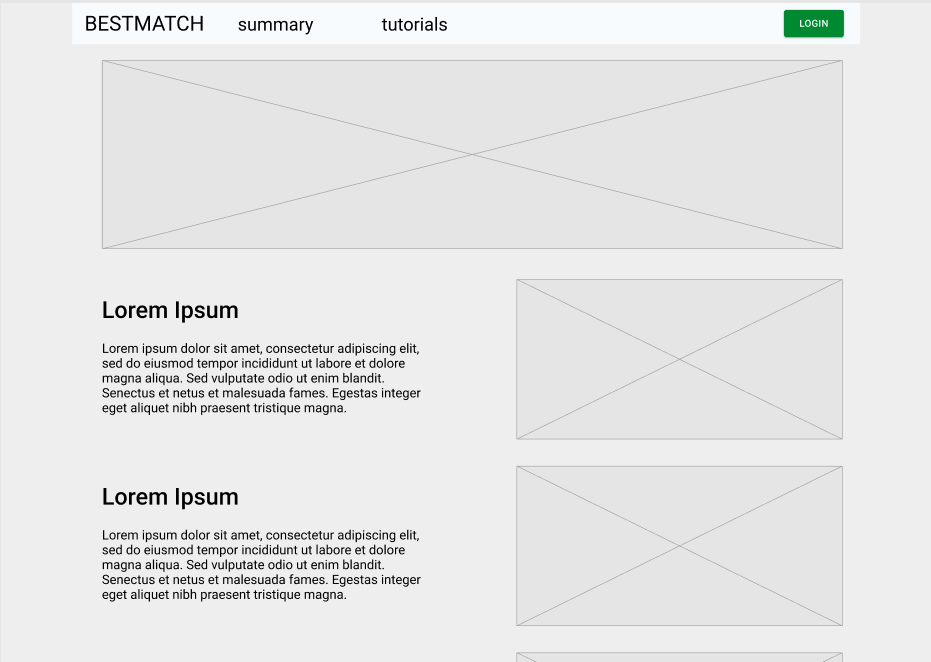
\includegraphics[width=\linewidth]{photo/student/tutorial.png}
          \end{center}
          \caption{หน้าคู่มือการใช้งาน}
          \label{fig:tutorial}
        \end{figure}
        \clearpage
  \item นักศึกษาเริ่มต้นใช้งานจะพบกับหน้าระบุคุณลักษณะของตนเอง
        \begin{figure}[h]
          \begin{center}
            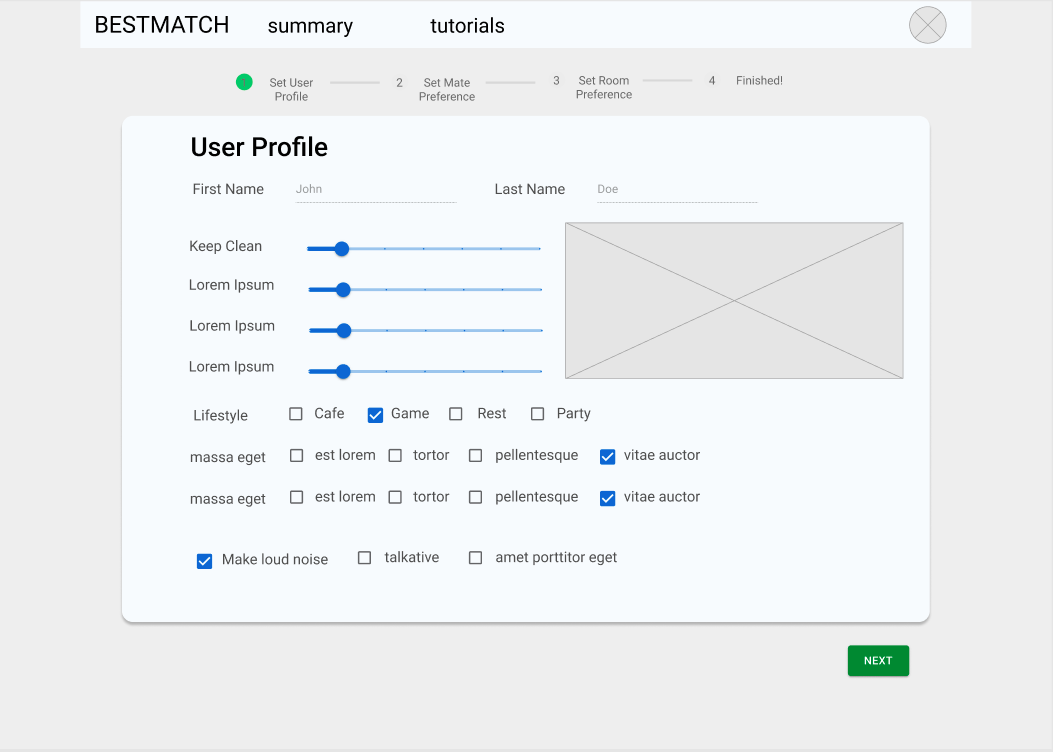
\includegraphics[width=\linewidth]{photo/student/user-profile.png}
          \end{center}
          \caption{หน้าระบุ $profile$ ของนักศึกษา}
          \label{fig:user-profile}
        \end{figure}
        \clearpage
  \item นักศึกษาระบุคุณลักษณะของผู้ร่วมอาศัยที่ต้องการ
        \begin{figure}[h]
          \begin{center}
            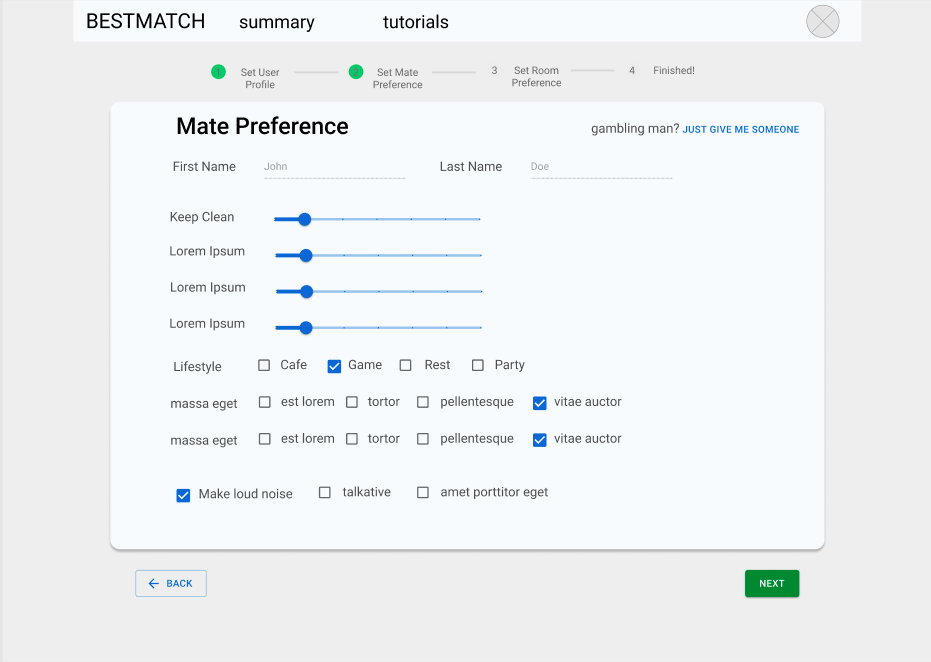
\includegraphics[width=\linewidth]{photo/student/mate-pref.png}
          \end{center}
          \caption{หน้าระบุ $matePref$ ของนักศึกษา}
          \label{fig:mate-pref}
        \end{figure}
        \clearpage
  \item นักศึกษาระบุห้องและหอพักที่ต้องการ
        \begin{figure}[h]
          \begin{center}
            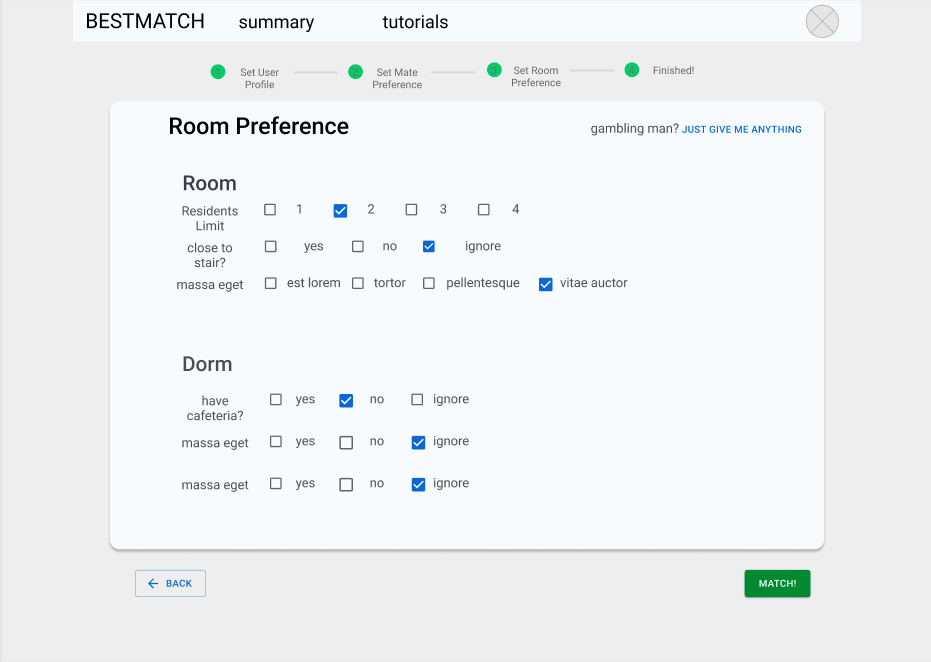
\includegraphics[width=\linewidth]{photo/student/room-pref.png}
          \end{center}
          \caption{หน้าระบุ $roomPref$ และ $dormPref$ ของนักศึกษา}
          \label{fig:room-pref}
        \end{figure}
        \clearpage
  \item นักศึกษาตรวจสอบคุณลักษณะของตนเอง และสามารถแก้ไขหากมีข้อผิดพลาดได้ด้วยปุ่ม edit
        \begin{figure}[h]
          \begin{center}
            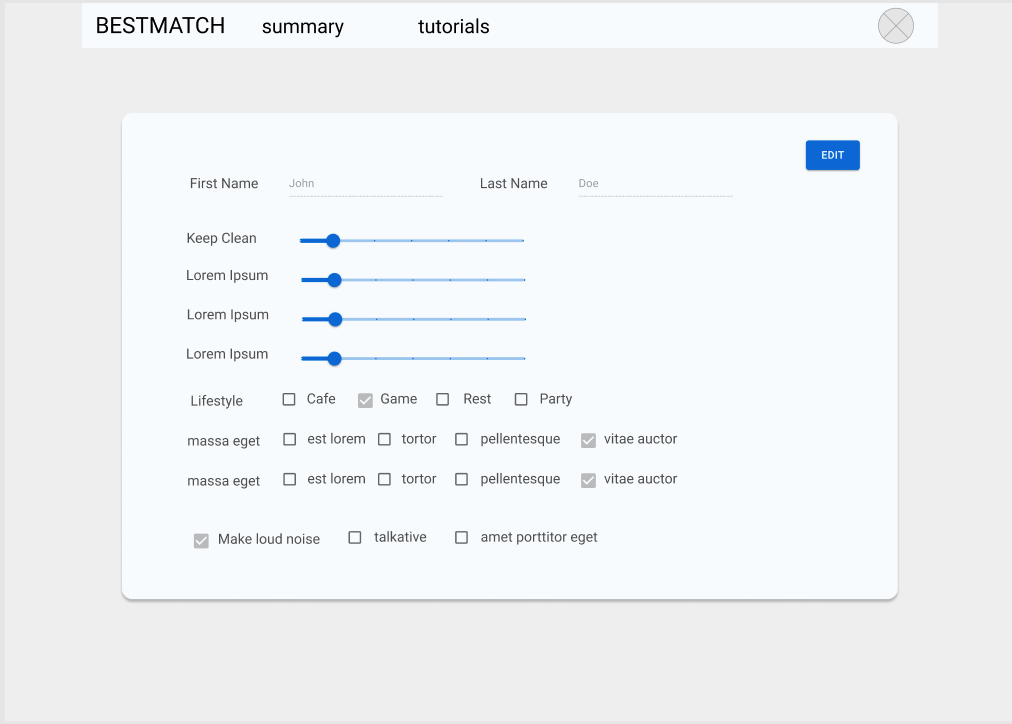
\includegraphics[width=\linewidth]{photo/student/profile.png}
          \end{center}
          \caption{หน้าโปรไฟล์}
          \label{fig:profile}
        \end{figure}
        \clearpage
  \item นักศึกษาตรวจสอบคุณลักษณะของผู้ร่วมอาศัยที่คาดว่าจะได้รับหลังจากระบบสิ้นสุดการประมวลผล
        \begin{figure}[h]
          \begin{center}
            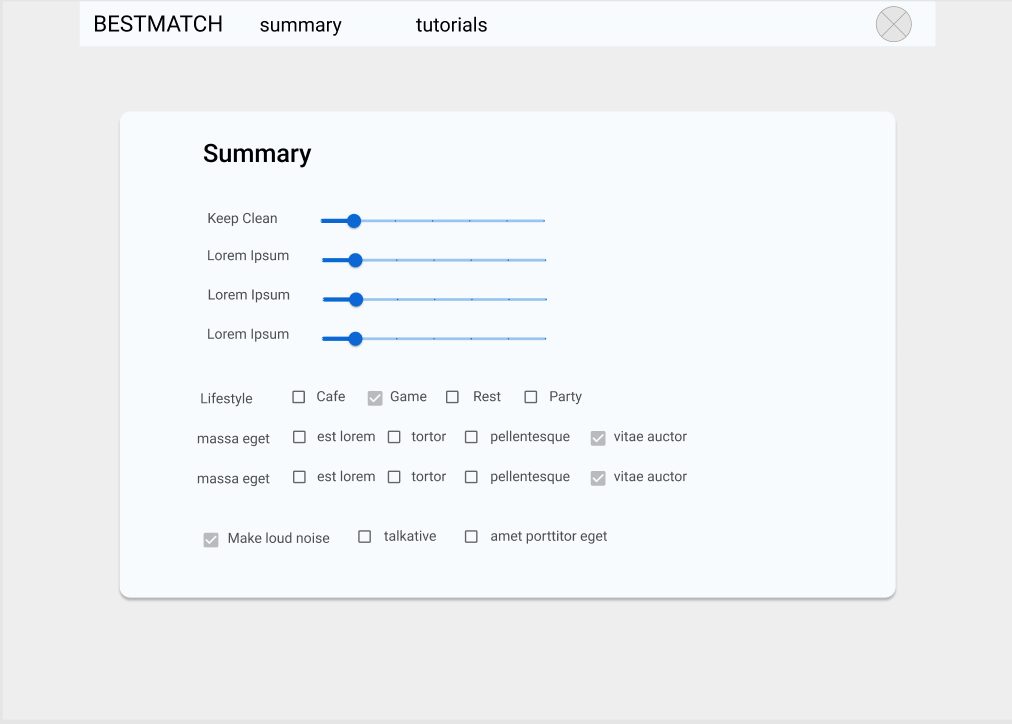
\includegraphics[width=\linewidth]{photo/student/summary.png}
          \end{center}
          \caption{หน้าสรุปผลคุณลักษณะที่ผู้ใช้ให้ความสนใจ}
          \label{fig:summary}
        \end{figure}
        % \item ระบบยืนยันตัวตน: ให้ผูู้ใช้ลงทะเบียนสมัครสมาชิกและเข้าสู่ระบบเพื่อที่จะสามารถใช้งานระบบต่างๆของระบบได้ต่อไป
        % \item ระบบการจัดอันดับคุณลักษณะ: ให้ผู้ใช้ที่ลงชื่อเข้าใช้แล้วเลือกคุณสมบัติของห้องและเพื่อนร่วมห้องที่ต้องการ
        % \item ระบบปรับจูนคุณลักษณะ: ระบบจะทำการนำโปรไฟล์ของบุคคลอื่นๆ มาแสดงให้ผู้ใช้เลือกว่า หากเป็นบุคคลที่มี
        %       คุณลักษณะตามโปรไฟล์ ผู้ใช้จะเลือกบุคคลดังกล่าวเป็นเพื่อนร่วมห้องหรือไม่ เพื่อคำนวณหาระดับความใส่ใจในคุณลักษณะต่างๆของผู้ใช้ 
        %       ตัวอย่างดังรูปที่~\ref{fig:finetune}
        % \item ระบบรายงานสรุปผล: แสดงความคืบหน้าว่า ณ ปัจจุบันผู้ใช้มีโอกาสจะได้จับคู่กับเพื่อนร่วมห้องที่มีคุณลักษณะอย่างไร
        %       และจะได้ห้องแบบใด 
        % \item ระบบคู่มือการใช้งาน: แสดงคู่มือการใช้งานของระบบสำหรับผู้ใช้ทั่วไป ไม่รวมผู้ใช้ที่เป็นผู้ดูแลระบบ
        % \item ระบบโปรไฟล์ผู้ใช้: ให้ผู้ใช้เข้าไปปรับแต่งคุณลักษณะของตนเองเพื่อนำไปใช้ในการจับคู่กับผู้อื่น
\end{enumerate}

% \subsection{ผู้ดูแล}
% ส่วนของผู้ดูแลนั้นยังไม่มีการออกแบบ แต่เบื้องต้นคาดว่าจะเป็นแบบ dashboard 1 หน้าดังรูป\ME{...}{ใส่รูปตัวอย่าง dashboard} ที่สามารถบริหารจัดการสิ่งต่างๆ ต่อไปนี้
% \begin{enumerate}
%   \item ผู้ดูแลเพิ่มลด และแก้ไขข้อมูลของหอพัก เพื่อนำข้อมูลไปใช้ในการระบุห้องที่เปิดให้จองในระบบ
%   \item ผู้ดูแลระบุรายการห้องพักที่ไม่เปิดให้จอง โดยใช้รูปแบบ และประเภทไฟล์ที่ระบบกำหนดเบื้องต้นคาดว่าให้ผู้ดูแลระบุเป็นรายการในการจัดการห้อง
%   \item ผู้ดูแลตั้งค่าวันที่เปิด--ปิดระบบ โดยผู้ดูแลสามารถตั้งค่าได้ด้วยหน้าต่างใช้งาน หรืออาจใช้ไฟล์ที่ระบุห้องพักระบุวันเปิด--ปิดเช่นกัน
        % \item ระบบจัดการเวลาเปิด--ปิดวันลงทะเบียน: ให้ผู้ดูแลระบบสามารถตั้งค่าเวลาเปิด--ปิด
        % วันลงทะเบียนของผู้ใช้ทั่วไป
        % \item ระบบจัดการฐานข้อมูลและการตั้งค่าหอพักที่ใช้ในการลงทะเบียน: ให้ผู้ดูแลหอพักสามารถเลือกจัดการห้องและหอที่จะเปิดให้ลงทะเบียนในระบบได้
        % โดยการกดปุ่มเพิ่มเพื่อเพิ่มหอพัก กดปุ่มแก้ไขเพื่อแก้ไขจำนวนและเลขห้องที่เปิดให้ลงทะเบียนในระบบของหอนั้นๆ และกดปุ่มลบเพื่อลบหอนั้นๆออกจากระบบลงทะเบียน
        % \item ระบบศูนย์รวมไฟล์แม่แบบของระบบลงทะเบียน: ให้ผู้ดูแลระบบสามารถเข้ามาดาวน์โหลดไฟล์แม่แบบที่ต้องใช้ในการจัดการระบบฐานข้อมูล\CIreply{mention template}
        % ยกตัวอย่างเช่น ไฟล์แม่แบบการตั้งค่าห้องพักที่จะเปิดให้ลงทะเบียน ภายในไฟล์จะมีฟอร์มที่มีหัวข้อที่ต้องกรอกจัดเตรียมไว้ให้แล้ว ซึ่งไฟล์ทั้งหมดจะเป็นไฟล์สกุล .csv
        % \begin{figure}[h]
        % \begin{center}
        % 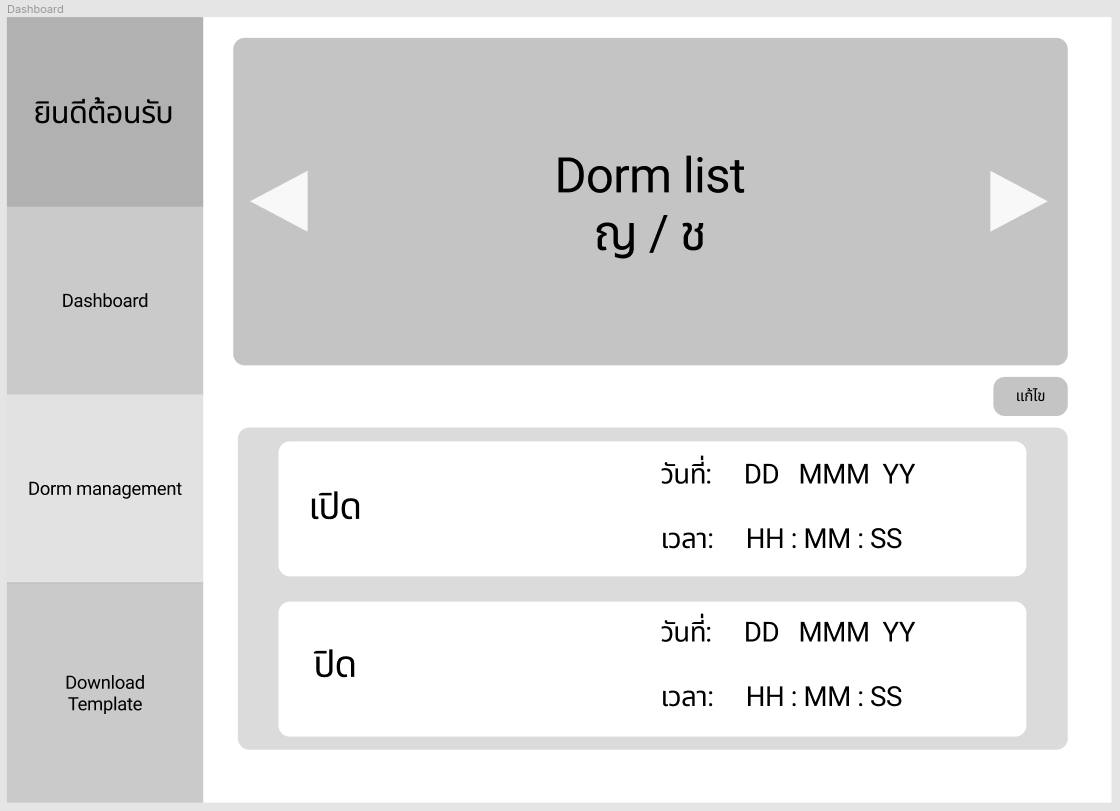
\includegraphics[width=\linewidth]{photo.old/adminDashboard.png}
        % \end{center}
        % \caption{หน้า homepage ของผู้ดูแลระบบ}
        % \label{fig:dashboard}
        % \end{figure}
        % \begin{figure}[h]
        % \begin{center}
        % 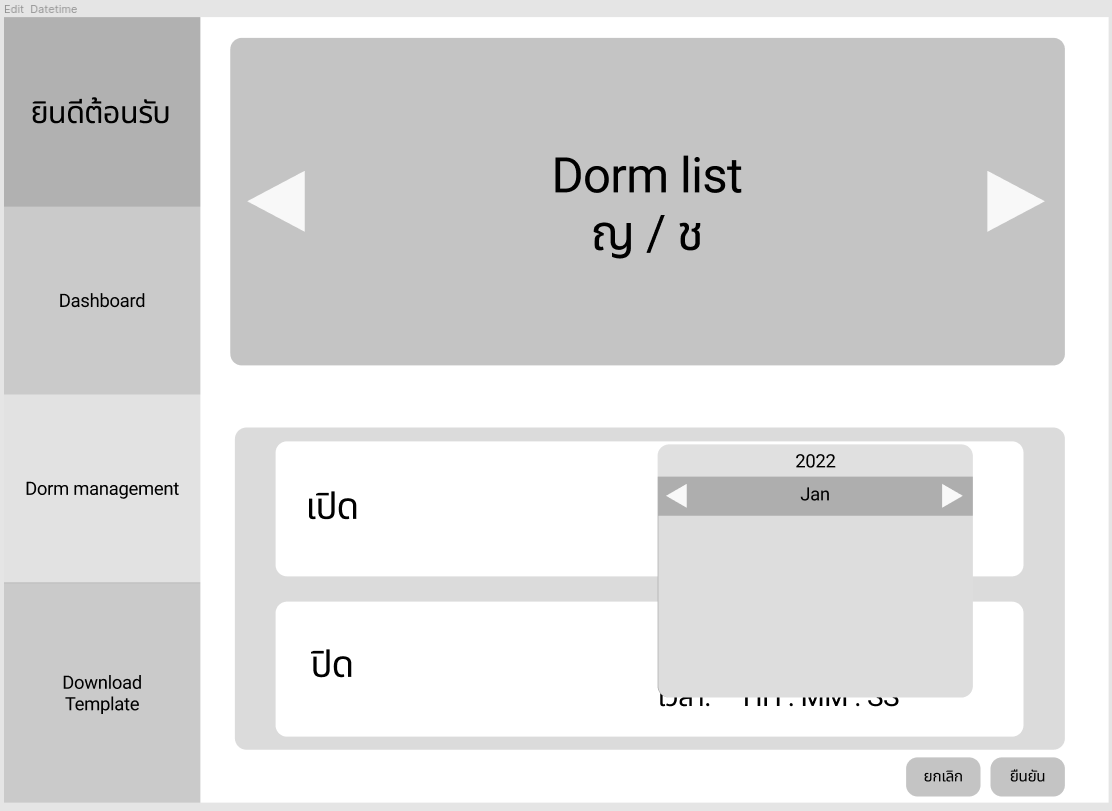
\includegraphics[width=\linewidth]{photo.old/datepicker.png}
        % \end{center}
        % \caption{ตัวอย่างการเปลี่ยนวันที่เปิด--ปิดระบบ}
        % \label{fig:datepicker}
        % \end{figure}
        % \begin{figure}[h]
        % \begin{center}
        % 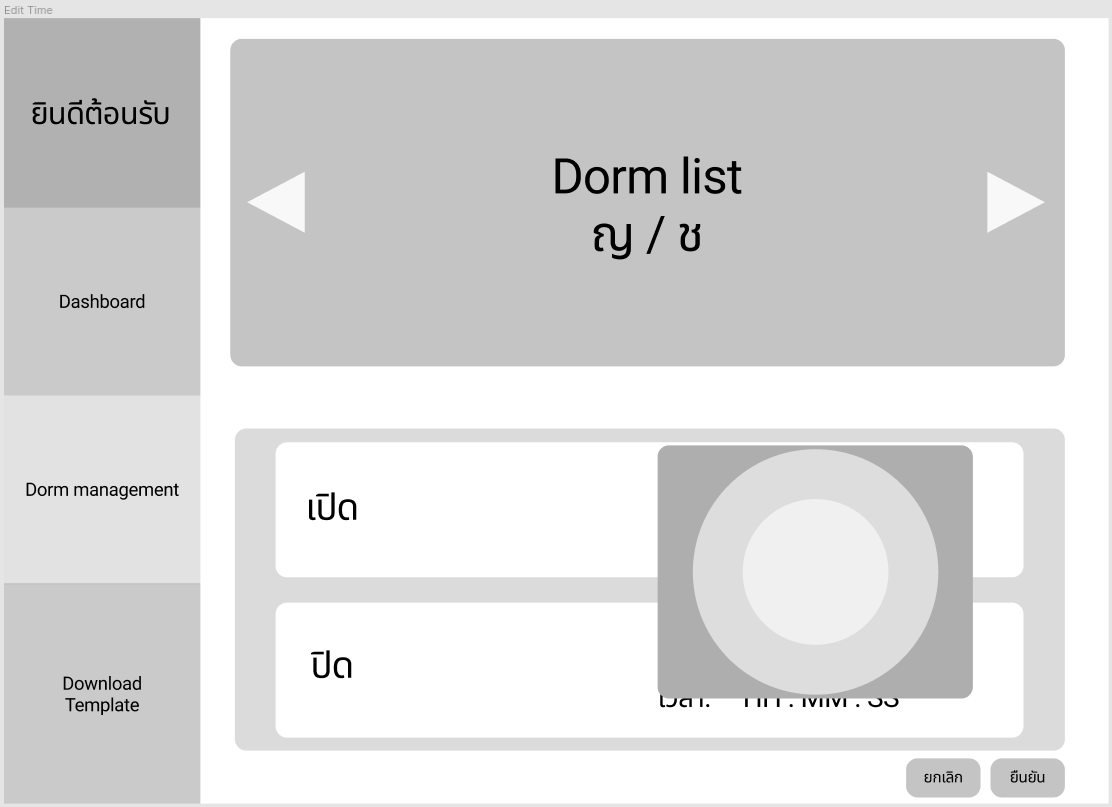
\includegraphics[width=\linewidth]{photo.old/timepicker.png}
        % \end{center}
        % \caption{ตัวอย่างการเปลี่ยนเวลาที่เปิด--ปิดระบบ}
        % \label{fig:timepicker}
        % \end{figure}
        % \begin{figure}[h]
        % \begin{center}
        % 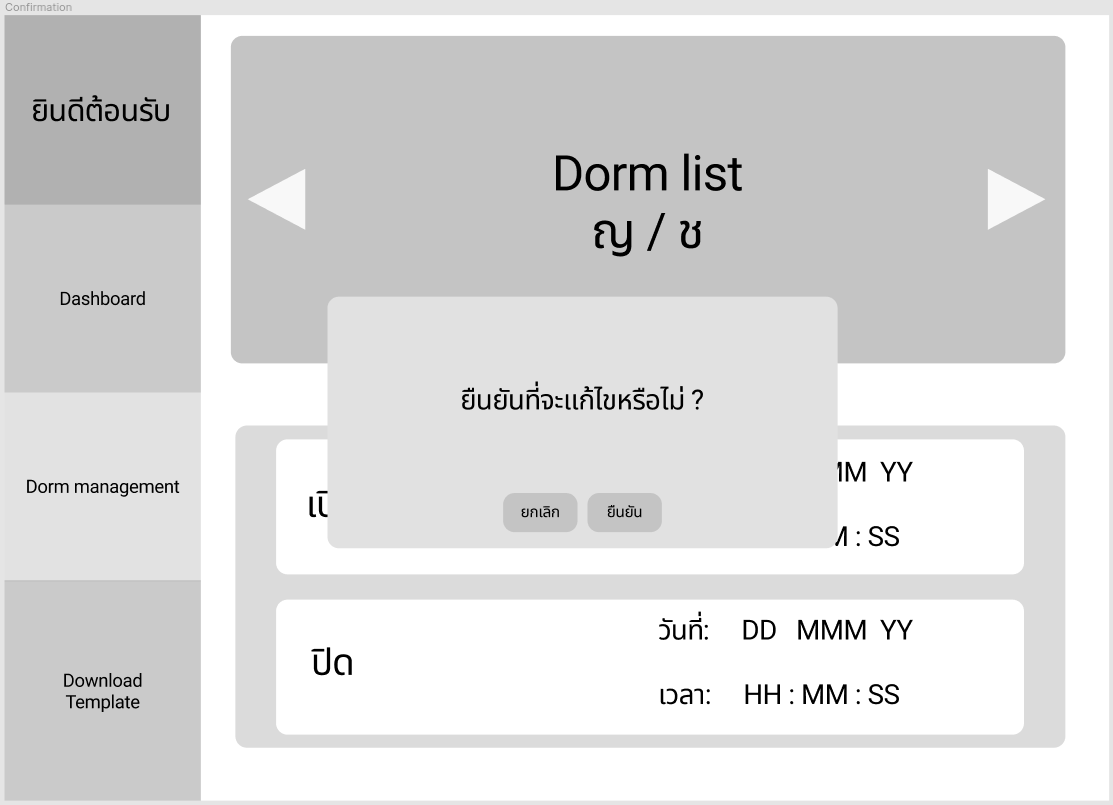
\includegraphics[width=\linewidth]{photo.old/confirmation.png}
        % \end{center}
        % \caption{ตัวอย่างแจ้งเตือนเพื่อยืนยันการตั้งค่า}
        % \label{fig:confirm-date-time}
        % \end{figure}
        
        % \clearpage
        % \begin{figure}[h]
        % \begin{center}
        % 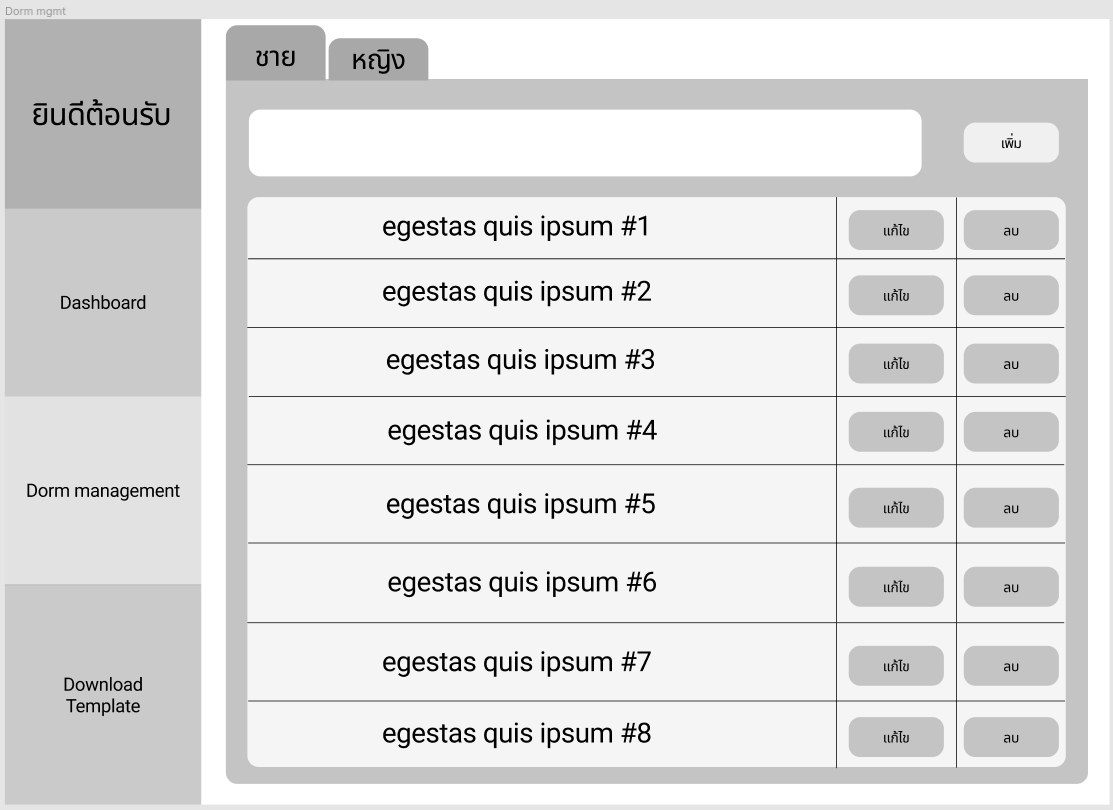
\includegraphics[width=\linewidth]{photo.old/dormmgmt.png}
        % \end{center}
        % \caption{หน้าการจัดการหอพักของระบบจอง}
        % \label{fig:mgmt}
        % \end{figure}
        % \begin{figure}[h]
        % \begin{center}
        % 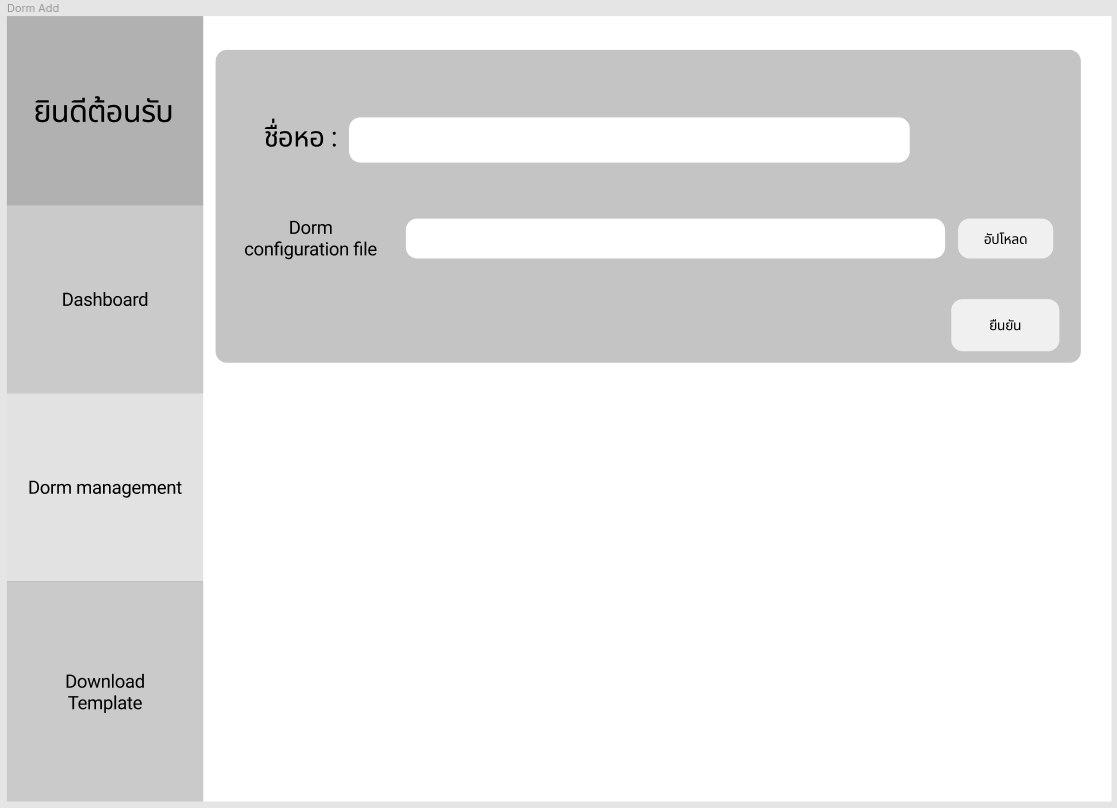
\includegraphics[width=\linewidth]{photo.old/dormadd.png}
        % \end{center}
        % \caption{หน้าการเพิ่มหอพักในระบบลงทะเบียน}
        % \label{fig:add-dorm}
        % \end{figure}
        % \begin{figure}[h]
        %   \begin{center}
        %   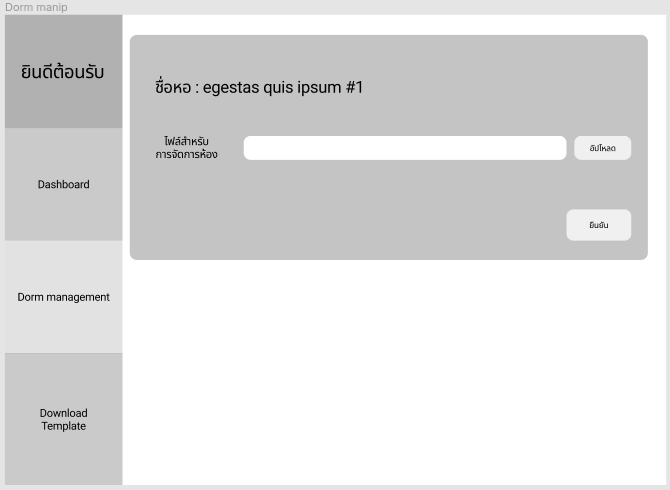
\includegraphics[width=\linewidth]{photo.old/roommgmt.png}
        %   \end{center}
        %   \caption{หน้าการจัดการเพิ่มลดห้องที่เปิดในระบบลงทะเบียน}
        %   \label{fig:room-mgmt}
        %   \end{figure}
        
        % \clearpage
        % \CIreply{ดาวน์โหลดไฟล์พวกนี้ไปเพื่ออะไร?}
        % \begin{figure}[h]
        % \begin{center}
        % 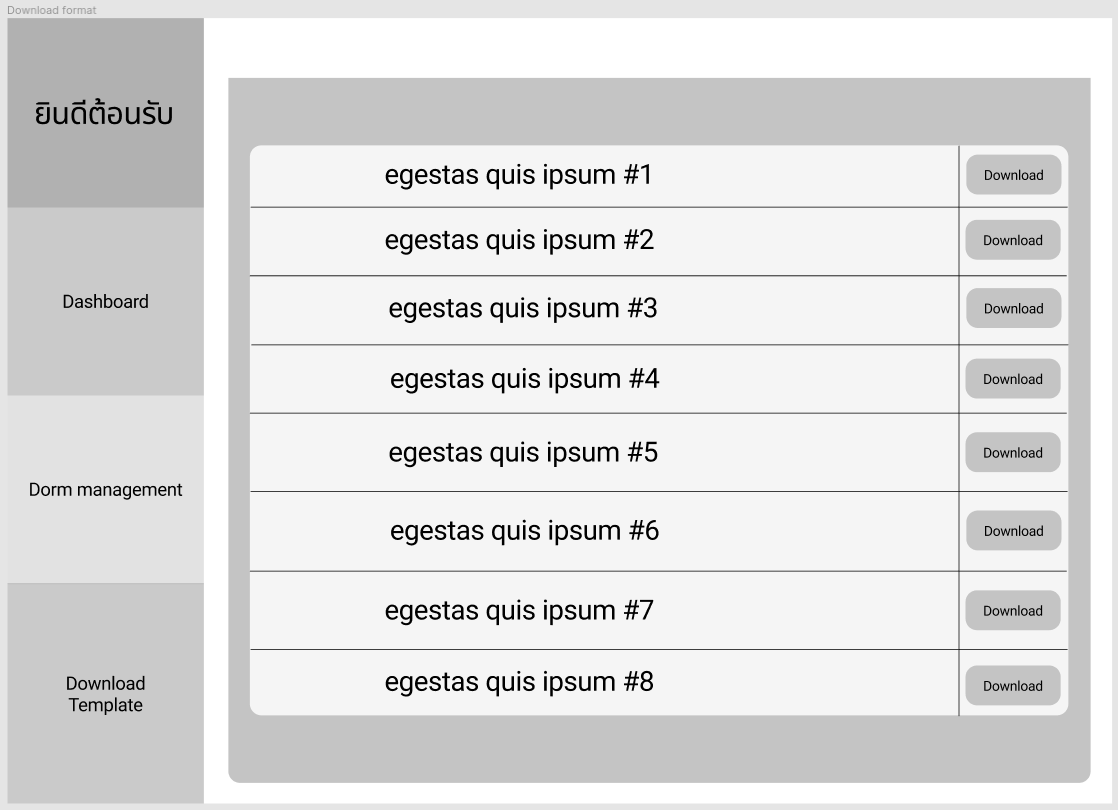
\includegraphics[width=\linewidth]{photo.old/format.png}
        % \end{center}
        % \caption{หน้าดาวน์โหลดไฟล์}
        % \label{fig:format-db}
        % \end{figure}
% \end{enumerate}
